

\chapter{Option pricing with transaction costs}\label{Chapter5}
%\blindtext
\minitoc% Creating an actual minitoc

\vspace{5em}

\section{Transaction cost models for the portfolio selection problem}
In the mathematical finance literature, the first application of stochastic optimal control theory to finance appears in the seminal paper \cite{Me69}.
This is the classical \emph{Merton optimal portfolio problem}, and is formulated as follows. An investor has a portfolio consisting of two assets, one ``risk free" $B$,
and the other ``risky" $S$. The portfolio follows the process
\begin{equation}\label{Merton_problem1}
 \begin{cases}
 dB_t &=  rB_t dt \\
 dS_t &=  S_t \left( \mu dt + \sigma dW_t \right),
\end{cases}
\end{equation} 
with $\mu>r$ and $\sigma>0$. If we denote with $\mathcal{W}_t = B_t + S_t$  the wealth at time $t$, and with $\pi_t$ the fraction of wealth invested in the risky asset, such that
$S_t = \pi_t \mathcal{W}_t$ and $B_t = (1-\pi_t) \mathcal{W}_t$. The model also takes into account the investor consumption $c(t) \geq 0$ for all $t$. 
The optimization problem can be formulated considering the utility function of the consumption and some terminal conditions, and consists in maximizing the objective function
\begin{equation}
 J(x;\pi,c) = \E_x \biggl[ \int_0^{T} e^{-\beta t} \mathcal{U}(c(t)) dt + g(T,\mathcal{W}_T) \biggr],
\end{equation}
where $\beta > 0$ and $\mathcal{U}: [0,\infty) \to \R$ is a concave and increasing utility function, such that $\mathcal{U}(0)=0$.
In the paper the function $g$ is called \emph{bequest valuation function} and is assumed to be concave.
We indicate the initial portfolio value with $x = (B_0,S_0)$. 
The wealth $\mathcal{W}$ takes values in $\OO = (0,\infty)$ and has state dynamics
\begin{equation}
 d \mathcal{W}_t = (1-\pi_t) \mathcal{W}_t r dt + \pi_t \mathcal{W}_t (\mu dt + \sigma dW_t) - c(t)dt.
\end{equation}
The control $\alpha_t$ is a two dimensional vector $(\alpha^1_t,\alpha^2_t) = (\pi_t,c_t)$, with values in $A = \R \times [0,\infty)$. 
This is a finite horizon problem with an objective function of type (\ref{cost_functional})
and HJB equation as in (\ref{DPE}). 
Even if in this case the control space $A$ is not compact, the supremum in (\ref{DPE}) is attained thanks to the concave structure of the problem.

Merton, using the utility $\mathcal{U}(c) = \frac{1}{\gamma} c^{\gamma}$ with $0<\gamma<1$ (of HARA type) obtained an explicit solution for the problem. In particular he found that 
the optimal control
\begin{equation}\label{Merton_policy}
  \pi^*_t = \frac{\mu-r}{(1-\gamma)\sigma^2}
\end{equation}
is a constant and does not depend on the state variables.  
This means that the optimal fraction of the risky and risk free assets in the portfolio is constant.
The line containing all the optimal points in the $(B,S)$ plane is the so called \textbf{Merton line}.

%In Chapter \ref{Chapter4} we have not considered infinite horizon control problems because they are not relevant for the thesis.
%The Merton optimal portfolio problem can be formulated as well in a finite time horizon setting, and removing the consumption rate. The objective function becomes
%\begin{equation}\label{Merton_problem2}
% J(t,x;\pi) = \E_{t,x} \biggl[ \mathcal{U}\biggl( \mathcal{W}^{\pi}(T) \biggr) \biggr] \quad \mbox{ for } \quad t \in [t_0,T].
%\end{equation}
%It turns out that the finite horizon solution is the same as the original infinite horizon Merton problem. The optimal policy is still given by formula (\ref{Merton_policy}).
%For the explicit derivation see for instance \cite{Pham}.

\noindent
The Merton portfolio selection problem is the first optimal portfolio problem solved by stochastic control theory methods. 
In \cite{Me71} the author extends the results to different utility functions.
All the successive models are generalizations of the Merton model, where by 
the word ``generalizations", we mean that under some particular choices of the parameters, the Merton problem is included in those models as a special case.
For what concerns this thesis, we review the main portfolio selection problems that have appeared in the literature, considering the presence of proportional transaction costs.
The first portfolio selection model with transaction costs and consumption was introduced by \cite{Co86} and then extended by \cite{DaNo90}. We refer to \cite{ShSo94}
for a viscosity solution approach to the same problem. 
Other important contributions are 
\cite{DaYi09}, \cite{Dai10}, \cite{LiuLo02}, \cite{LiuLo07}, \cite{BKR01}, \cite{OkSu01}, \cite{Kab16} where the last four articles use Lévy processes to model the stock dynamics. 
All the cited works are portfolio optimization models formulated as infinite horizon problems, and do not involve the pricing of the options.

Further assumptions are needed when the portfolio process is introduced for the purpose of pricing a derivative contract.
The main contributions on option pricing with transaction costs, using the \emph{indifference pricing} approach are
\cite{HoNe89} and \cite{DaPaZa93} (DPZ). The problem is formalized as a finite horizon singular stochastic control problem.
In this section we present the DPZ model, which is the building block of this thesis, and then extend it following the framework introduced by \cite{Kab16}, 
who consider the stock dynamics described by Lévy processes.
The main results of this Chapter are collected in the paper \cite{Canta}.


\subsection{Davis - Panas - Zariphopoulou (DPZ)}\label{DPZ_sec}

This is the market model with proportional transaction costs presented in \cite{DaPaZa93}. 
The authors consider a portfolio composed by one risk-free asset $B$ (bank account) paying a fixed interest rate $r > 0$ and a stock $S$. 
The symbol $Y$ denotes the number of shares of the stock $S$ that the investor holds. 
The state of the portfolio at time $t\in [t_0,T]$ is $(B^{\pi}_t,Y^{\pi}_t,S_t)$, and is the solution of the following the SDE:
\begin{equation}\label{DPZ_porfolio_dynamics}
 \begin{cases}
 dB^{\pi}_t &=  rB^{\pi}_t dt - (1+\theta_b)S_t dL_t + (1-\theta_s) S_t dM_t \\
 dY^{\pi}_t &=  dL_t - dM_t \\
 dS_t &=  S_t \left( \mu dt + \sigma dW_t \right).
\end{cases}
\end{equation} 
for a particular strategy $\{\pi_t\}_{t \in [t_0,T]} := \{(L_t,M_t)\}_{t \in [t_0,T]}$.
The parameters $\theta_b$, $\theta_s \geq 0$ are the proportional transaction costs when buying and selling respectively.
This portfolio equation is a generalization of the portfolio in the Merton problem (\ref{Merton_problem1}), 
where there is a new state variable $Y$ and the action of the controls is represented with a different approach.
The control process $\{\pi_t\}_{t \in [t_0,T]} := \{(L_t,M_t)\}_{t \in [t_0,T]}$ represents the trading strategy and indicates the 
cumulative number of shares bought and sold respectively in $[t_0,T]$.
The strategy $\pi(t)$ is a cádlág, $\mathcal{F}_t$-progressively measurable, nondecreasing process with bounded variation in every finite time interval and such that
$ \pi(t_0^-) = ( L(t_0^-) , M(t_0^-) ) = (0,0) $, allowing for an initial transaction at $t_0$.\\
In the discontinuity points of $L_t$ and $M_t$ we indicate the process variation with $\Delta L_t= L(t)-L(t^-)$ and $\Delta M_t= M(t)-M(t^-)$.

% In order to understand better the mechanism, let us make a recap:
% \begin{itemize}
%  \item Variation in the number of shares:
%  $$\Delta Y^{\pi}_t =  \underbrace{\Delta L_t}_{\mbox{shares bought}} - \underbrace{\Delta M_t}_{\mbox{shares sold}} $$
%  \item Variation in the bank account:
%  $$ \Delta B^{\pi}_t =  - \underbrace{(1+\theta_b)S_t}_{\mbox{adjusted price}} \Delta L_t + \underbrace{(1-\theta_s) S_t}_{\mbox{adjusted price}} \Delta M_t $$
% \end{itemize}
% we can identify this problem as a singular stochastic control problem as described in Chapter \ref{singular_control}.


\begin{Definition}
We define the \textbf{cash value} function $c(y,s)$ as the value in cash when the shares in the portfolio are liquidated, i.e.  
long positions are sold and short positions are covered.
\begin{equation}\label{cost_function}
c(y,s) = \begin{cases} 
(1+\theta_b)ys, & \mbox{if } y\leq 0 \\ 
(1-\theta_s)ys, & \mbox{if } y>0 . 
\end{cases} 
\end{equation} 
\end{Definition}
\begin{Definition}
For $t\in [t_0,T]$, we define the \textbf{total wealth} process:
\begin{equation}\label{wealth_process}
 \mathcal{W}^{\pi}_t = B^{\pi}_t + c(Y^{\pi}_t,S_t).
\end{equation} 
\end{Definition}
We say that a portfolio is solvent if the portfolio's wealth $\mathcal{W}_t$ is greater than a fixed constant $-C$, with 
$C\geq0$ that may depend on the initial wealth and on the parameters in (\ref{DPZ_porfolio_dynamics}). 
This constant may be interpreted as the \emph{credit availability} of the investor.
\begin{Definition}
We define the \textbf{solvency region}:
\begin{equation}\label{solvency_region}
 \mathcal{S} := \biggl\{ (b,y,s) \in \R \times \R \times \R^+ : b + c(y,s) > -C  \biggr\}.
\end{equation} 
\end{Definition}
\begin{Definition}\label{admissible_strategies1}
The set of \textbf{admissible trading strategies} $\Pi(t_0,b,y,s)$, is defined   
as the set of all right-continuous, nondecreasing, $\mathcal{F}_t$-progressively measurable processes  
$\{\pi_t\}_{t \in [t_0,T]}$, such that $(B^\pi(t),Y^\pi(t),S(t))$ is a solution of (\ref{DPZ_porfolio_dynamics}) with initial values $(B^\pi_{t_0} = b, Y^\pi_{t_0} = y, S_{t_0} = s)$, 
and 
\begin{equation}
 \mathcal{W}^{\pi}_t \in \mathcal{S}
\end{equation}
for $t \in [t_0,T]$ almost surely.
\end{Definition}


\subsubsection{Utility maximization}

The objective of the investor is to maximize the expected utility of the wealth at time $T$ over all the admissible
strategies. This expectation is conditioned on the initial value of cash $B_0$, number of shares $Y_0$ and value of the
stock $S_0$.
The value function of the maximization problem is:
\begin{equation}\label{DPZ_max_probl0}
V^0(t_0,B_0,Y_0,S_0) = \sup_{\pi \in \Pi(B_0)} \;  \E_{B_0,Y_0,S_0}\biggl[ 
            \mathcal{U}(\mathcal{W}^0_T) \biggr], 
\end{equation}
where $\mathcal{U}: (-C,\infty) \to \R$ is a concave and increasing utility function, such that $\mathcal{U}(0)=0$. 
Here we use the superscript ``$0$'' to indicate that this is the case of a portfolio with \emph{zero options}. 
\begin{Remark}
It is important to stress that the utility function
has to be defined also for negative numbers, and this requirement excludes the logarithmic utility for instance.
\end{Remark}

Assume an investor builds a portfolio with cash, shares of a stock and in addition he sells or purchases a 
European call option written on the same stock, with strike price $K$ and expiration date $T$.
This means that at time $t_0$ the initial amount in the cash account increases by the option's value $p^w$ (in the writer case), 
or decreases by $p^b$ (in the buyer case). 
We define the wealth processes for the writer and buyer portfolios respectively:
\begin{itemize}
  \item Writer: 
  \begin{equation}\label{wealth_writer}
   \mathcal{W}^w_t =  B_t + c(Y_t,S_t) \mathbbm{1}_{\{t\leq T,\, c(1,S_T) \leq K\}} +
  \biggl( c\bigl( Y_t-1,S_t \bigr) + K \biggr) \mathbbm{1}_{\{t=T,\, c(1,S_T)>K\}}.
  \end{equation}
  \item Buyer: 
  \begin{equation}\label{wealth_buyer}
   \mathcal{W}^b_t = B_t + c(Y_t,S_t) \mathbbm{1}_{\{t\leq T,\, c(1,S_T) \leq K\}} +
  \biggl( c\bigl( Y_t+1,S_t \bigr) - K \biggr) \mathbbm{1}_{\{t=T,\, c(1,S_T)>K\}}.
  \end{equation}
\end{itemize}
In the case the option is exercised, $c(1,S_T) >K$, the buyer pays the writer the strike $K$ in cash, 
and the writer delivers one share to the buyer.
In a market with transaction costs 
the real value (in cash) of a share is given by the bilinear cash cost function (\ref{cost_function}). 
The buyer of the option does not exercise
when $S_T > K$, but when $c(1,S_T) = S_T (1-\theta_s) > K$.
The \emph{solvency regions} for the writer/buyer are:
\begin{itemize}
  \item  \begin{equation}\label{solvency_writer}
 \mathcal{S}^w = \biggl\{ (B_t,Y_t,S_t) \in \R \times \R \times \R^+ : \mathcal{W}^w_t  > -C  \biggr\}          
         \end{equation}
 
  \item \begin{equation}\label{solvency_buyer}
  \mathcal{S}^b = \biggl\{ (B_t,Y_t,S_t) \in \R \times \R \times \R^+ : \mathcal{W}^b_t  > -C  \biggr\}.        
        \end{equation}
\end{itemize}
The investor wishes to maximize the expected utility of the wealth of his portfolio. 
\begin{equation}\label{DPZ_max_probl1}
V^j(t_0,B_0^j,Y_0,S_0) = \sup_{\pi \in \Pi(B_0)} \; \E_{B_0^j,Y_0,S_0}\biggl[ 
            \mathcal{U}(\mathcal{W}^j_T) \; \biggr], 
\end{equation}
where $B_0^j$ is the initial cash amount in the writer $(j=w)$ or buyer $(j=b)$ portfolio and can assume the two values $B_0+p^w$ and $B_0-p^b$. 
The exit time $\tau^j$ is associated with the writer/buyer solvency region $ \mathcal{S}^j$, respectively for $j=w,b$.

With this model we can compute two option prices: the price for the writer and the price for the buyer.
These prices are defined, respectively, as the amount required to get the same maximal expected utility of the wealth of 
the option-free portfolio.
To compute the option price, 
it is necessary to solve two portfolio optimization problems: the problem without the option
and the problem with the option.
We define the 
\begin{itemize}
 \item Writer price:
 \begin{equation}\label{writer_p}
  V^0(t_0,B_0,Y_0,S_0) = V^w(t_0,B_0+p^w,Y_0,S_0)
 \end{equation}
 \item Buyer price:
 \begin{equation}\label{buyer_p}
  V^0(t_0,B_0,Y_0,S_0) = V^b(t_0,B_0-p^b,Y_0,S_0)
 \end{equation}
\end{itemize}
The prices $p^w$ and $p^b$ can be obtained implicitly by these conditions.


\subsubsection{HJB Equation}\label{subsec_HJB}

In view of the general theory of stochastic control problems and in particular singular control problems introduced in Chapter \ref{Chapter4}, we can make a small summary of the 
DPZ model equations and derive the dynamic programming equation of the problem.
We write the state equation (\ref{DPZ_porfolio_dynamics}) for $X_t = (B_t,Y_t,S_t)$ in matrix form 
\begin{align}\label{DPZ_porfolio_dynamicsM}
d X_t
=& 
 d \left(
\begin{array}{l}
B_t\\
Y_t\\
S_t
\end{array} \right) \\ \nonumber
  =&  \left( \begin{array}{l}
r B_t\\
0\\
\mu S_{t}
\end{array} \right)
dt +  \left( \begin{array}{l}
0\\
0\\
\sigma S_{t}
\end{array} \right) dW_t \\ \nonumber
&+ \left( \begin{array}{l}
-S_{t}(1+\sigma_b) \\
1\\
0
\end{array} \right) dL_t
+ \left( \begin{array}{l}
S_{t}(1-\sigma_s) \\
-1\\
0
\end{array} \right) dM_t.
\end{align}
The state space takes values in $\OO$ corresponding to the solvency region $\SI$.
The cost function (\ref{cost_functional}) corresponds to 
\begin{equation}
V(t_0,X_0; \pi) = \sup_{\pi \in \Pi(B_0)} \;  \E_{X_0}\biggl[ 
            \mathcal{U}(\mathcal{W}^j_T) \biggr], 
\end{equation}
with $j=w,b,0$ depending on the specific considered problem. Here the running cost is zero, and the are only terminal costs. 

In order to identify our problem in the class of general singular problems with dynamics described by (\ref{controlled_SDE}) with singular control as in (\ref{linear_control}), 
let us assume that 
$dL_t \ll dt$ and $dM_t \ll dt$, i.e. the controls are absolutely continuous. We can write
\begin{equation}\label{absolute_cont_controls}
 L(t) = \int_{t_0}^t l(s) ds \quad \mbox{ and } \quad M(t) = \int_{t_0}^t m(s) ds, 
\end{equation}
where $0 \leq l(s) \leq k$ and $0 \leq m(s) \leq k$ with $k<\infty$.
Under this assumption the state dynamics (\ref{DPZ_porfolio_dynamics}) becomes
\begin{equation}\label{DPZ_porfolio_dynamics2}
 \begin{cases}
 dB^{\pi}_t &=  rB_t dt - (1+\theta_b)S_t \,l_t \, dt + (1-\theta_s) S_t \, m_t\, dt \\
 dY^{\pi}_t &=  \bigl( l_t - m_t \bigr) dt \\
 dS_t &=  S_t \left( \mu dt + \sigma dW_t \right).
\end{cases}
\end{equation} 
This state dynamics is affected linearly by the control as in Eq. (\ref{linear_control}).
\begin{align}\label{DPZ_porfolio_dynamicsM2}
d \left(
\begin{array}{l}
B_t\\
Y_t\\
S_t
\end{array} \right)
  =&  \left( \begin{array}{l}
r B_t\\
0\\
\mu S_{t}
\end{array} \right)
dt +  \left( \begin{array}{l}
0\\
0\\
\sigma S_{t}
\end{array} \right) dW_t \\ \nonumber
&+ \left[ \underbrace{\left( \begin{array}{l}
-S_{t}(1+\sigma_b) \\
1\\
0
\end{array} \right)l_t}_{\alpha_1(t)}
+ \underbrace{\left( \begin{array}{l}
S_{t}(1-\sigma_s) \\
-1\\
0
\end{array} \right) m_t}_{\alpha_2(t)} \right] dt.
\end{align}
The control process $\alpha(\cdot) = (\alpha_1(\cdot), \alpha_2(\cdot))$ is an element of the set $\mathcal{A}^k$,
which is the subset of $\Pi(B_0)$ containing all the controls $L(t)$ and $M(t)$ that are absolutely continuous. 
The process $\alpha_t$ assumes values in 
\begin{equation}
A^k = \biggl\{ \bigl(-S_{t}(1+\sigma_b),1,0) \cdot l \; : \; 0<l<k \biggr\} \bigcup \biggl\{ \bigl(S_{t}(1-\sigma_s),-1,0\bigr)\cdot m \; : \; 0<m<k \biggr\}.  
\end{equation}
The set $A$ considered in (\ref{unbounded_set}) is unbounded. We can approach the unbounded set by taking the limit for $k\to \infty$, such that    
$A^k \to A$ (see the remark \ref{RemarkDPZ} ) with $A$ defined as:
\begin{equation}
A = \biggl\{ \bigl(-S_{t}(1+\sigma_b),1,0) \cdot l \; : \; l>0 \biggr\} \bigcup \biggl\{ \bigl(S_{t}(1-\sigma_s),-1,0\bigr)\cdot m \; : \; m>0 \biggr\}. 
\end{equation}
According to the equation (\ref{variational_inequality}), the HJB equation of the singular control problem is a variational inequality. Here we have
\begin{itemize}
 \item $ D_x V(t,x) = \left( \frac{\partial V(t,b,y,s)}{\partial b}, \frac{\partial V(t,b,y,s)}{\partial y}, \frac{\partial V(t,b,y,s)}{\partial s} \right) $
 \item $H(p) = \sup_{a \in \hat K} \bigl( a\cdot p \bigr) \quad \mbox{ and define } \quad \hat K = \{ a \in A: |l|=|m|=1 \}$
 \item $H \bigl( D_x V(t,x) \bigr) = \max \biggl\{ \frac{\partial V}{\partial y}-(1+\theta_b) s \frac{\partial V}{\partial b} ,
 -\bigl( \frac{\partial V}{\partial y} -(1-\theta_s)s \frac{\partial V}{\partial b} \bigr) \biggr\} $
\end{itemize}
The resulting HJB equation is
\begin{align}\label{DPZ_HJB}
& \max \; \biggl\{ \; \frac{\partial V}{\partial t} + rb\frac{\partial V}{\partial b} 
+ \mu s \frac{\partial V}{\partial s} + \frac{1}{2}\sigma^2 s^2 \frac{\partial^2 V}{\partial s^2}, \\ \nonumber
& \;  \frac{\partial V}{\partial y}-(1+\theta_b) s \frac{\partial V}{\partial b} \; 
, \; -\biggl(\frac{\partial V}{\partial y}-(1-\theta_s)s \frac{\partial V}{\partial b} \biggr) \biggr\} = 0, 
\end{align}
for $(t,b,y,s) \in [t_0,T] \times \SI$.

\noindent
The variational inequality (\ref{DPZ_HJB}) says that the maximum of three operators is equal to zero.
This feature can be interpreted better if we consider the state space divided into three different regions: the \textbf{Buy}, the \textbf{Sell}
and the \textbf{No Transaction} (NT) regions.
\begin{itemize}
 \item \textbf{Buy}
  \begin{equation*}
   \begin{cases}
     & \frac{\partial V}{\partial t} + rb\frac{\partial V}{\partial b} + \mu s \frac{\partial V}{\partial s} + \frac{1}{2}\sigma^2 s^2 \frac{\partial^2 V}{\partial s^2} \leq 0\\ 
     & \frac{\partial V}{\partial y}-(1+\theta_b) s \frac{\partial V}{\partial b} = 0 \\
     & -\biggl(\frac{\partial V}{\partial y}-(1-\theta_s)s \frac{\partial V}{\partial b} \biggr) < 0.
   \end{cases}
  \end{equation*}
 \item \textbf{Sell}
  \begin{equation*}
   \begin{cases}
     & \frac{\partial V}{\partial t} + rb\frac{\partial V}{\partial b} + \mu s \frac{\partial V}{\partial s} + \frac{1}{2}\sigma^2 s^2 \frac{\partial^2 V}{\partial s^2} \leq 0 \\ 
     & \frac{\partial V}{\partial y}-(1+\theta_b) s \frac{\partial V}{\partial b} < 0 \\
     & -\biggl(\frac{\partial V}{\partial y}-(1-\theta_s)s \frac{\partial V}{\partial b} \biggr) = 0.
   \end{cases}
  \end{equation*}
 \item \textbf{No Transaction}
  \begin{equation*}
   \begin{cases}
     & \frac{\partial V}{\partial t} + rb\frac{\partial V}{\partial b} + \mu s \frac{\partial V}{\partial s} + \frac{1}{2}\sigma^2 s^2 \frac{\partial^2 V}{\partial s^2} = 0 \\ 
     & \frac{\partial V}{\partial y}-(1+\theta_b) s \frac{\partial V}{\partial b} < 0 \\
     & -\biggl(\frac{\partial V}{\partial y}-(1-\theta_s)s \frac{\partial V}{\partial b} \biggr) < 0.
   \end{cases}
  \end{equation*}
\end{itemize}
The optimization problem is a free boundary problem, and its solution consists of finding the value function $V$ and the 
optimal boundaries that divide the three regions.
The boundaries completely characterize the investor's trading strategy.
The optimal strategy consists in keeping the portfolio process inside the NT region. 
If the portfolio process crosses the NT region, the optimal strategy is to trade in order to bring back the portfolio
on the boundary with the NT region.
We can argue that Buy and Sell regions are separated by the NT region, 
since it is clearly not optimal to buy and sell a stock at the same time.
In the Buy and Sell regions the value functions remain constant along the directions of the trades.
We have respectively:
\begin{itemize}
 \item Buy: \hspace{2em} $V(t,b,y,s) = V(t,b-s(1+\theta_b)\Delta L^*_t,y+\Delta L_t,s).$
 \item Sell: \hspace{2em} $ V(t,b,y,s) = V(t,b+s(1-\theta_s)\Delta M^*_t,y-\Delta M_t,s).$
\end{itemize}
where $\Delta L^*_t$ and $\Delta M^*_t$ are the optimal number of shares respectively bought or sold in the trade.
The second and third terms in the HJB equation (\ref{DPZ_HJB}) are the gradients of the value function along the 
trading directions from the Buy and Sell regions to the NT boundaries.
In the NT region the portfolio evolves according to the portfolio equation (\ref{DPZ_porfolio_dynamics}), with $dL=dM=0$.
Therefore the number of shares remains constant as long as the portfolio stays in the NT region.
If we assume that the process does not leave the NT region in the (small) time interval $\Delta t$, 
by the dynamic programming principle we can write the value function simply as:
\begin{equation}\label{DPP_NO_trans}
 V(t,b,y,s) = \E_{b,y,s} \biggl[ V(t+\Delta t, b+\Delta B, y, s+\Delta S ) \biggr] 
\end{equation}
where we indicate with $\Delta B=b\,r\Delta t$ and $\Delta S$ the change in the cash account 
and in the stock price after $\Delta t$. The formula (\ref{DPP_NO_trans}) is the integral representation of the first operator in Eq. (\ref{DPZ_HJB}).
This can be proved easily by applying the Itô lemma, and sending $\Delta t \to 0$.


\begin{Remark}\label{RemarkDPZ}
 In the theory of singular stochastic control, it is common to consider the right-continuous (or left-continuous) control as the point-wise limit of a sequence of continuous function.
 The theory presented in Chapter \ref{Chapter4}, considers directly a linear control, taking values in an unbounded set, in the coefficients of the SDE (Eqs. (\ref{linear_control}) 
 and (\ref{unbounded_set})). 
 However, this is equivalent to consider the limit of a sequence of absolute continuous controls, as presented for instance in (\cite{DaPaZa93}). 
 For a formal convergence proof we refer to \cite{BuRo06}, where the authors prove that when $k\to \infty$ and $A^k \to A$, then $\mathcal{A}^k \to \Pi(B_0)$.  
 In the same paper the authors also prove the existence of the optimal control for diffusion processes.
\end{Remark}



\subsection{DPZ with jumps}\label{DPZ_j_sec}


The objective of this thesis is to extend the DPZ model in order to include jumps in the dynamics. Let us assume that the stock follows an exponential Lévy process with SDE 
as in \ref{exp_sde2}:
\begin{equation}\label{porfolio_dynamics}
 \begin{cases}
 dB^{\pi}_t &=  rB_t dt - (1+\theta_b)S_t dL_t + (1-\theta_s) S_t dM_t \\
 dY^{\pi}_t &=  dL_t - dM_t \\
 dS_t &=  S_t \left( \mu dt + \sigma dW_t + \int_{\R} (e^z-1) \tilde N(dt,dz) \right).
\end{cases}
\end{equation} 
This is analogous to the portfolio process (\ref{DPZ_porfolio_dynamics}), where only the dynamics of $S_t$ is modified and all the other components are the same.
A further difference here is that we choose the
strategy $\pi(t) = (L(t),M(t))$ to be $\mathcal{F}_t$-progressively measurable, nondecreasing with bounded variation and left-continuous. This choice is made according to the model 
developed in \cite{ShSo94}, \cite{FlemingSoner} and \cite{BaSo98}.
At time $t_0$ the control is $ \pi(t_0) = ( L(t_0) , M(t_0) ) = (0,0) $.
The definitions of cash value (\ref{cost_function}), of total wealth (\ref{wealth_process}), (\ref{wealth_buyer}), (\ref{wealth_writer}) and the solvency regions
(\ref{solvency_region}), (\ref{solvency_buyer}), (\ref{solvency_writer}) are kept the same. However the set of admissible trading strategy needs to be changed.

Control processes satisfy $L(t) = L(t^-)$ and $M(t) = M(t^-)$.
In the discontinuous points of $L(t)$ and $M(t)$, we indicate the process variation with $\Delta L_t= L(t^+)-L(t)$ and $\Delta M_t= M(t^+)-M(t)$.\\
\begin{figure}[t!]
 \centering
 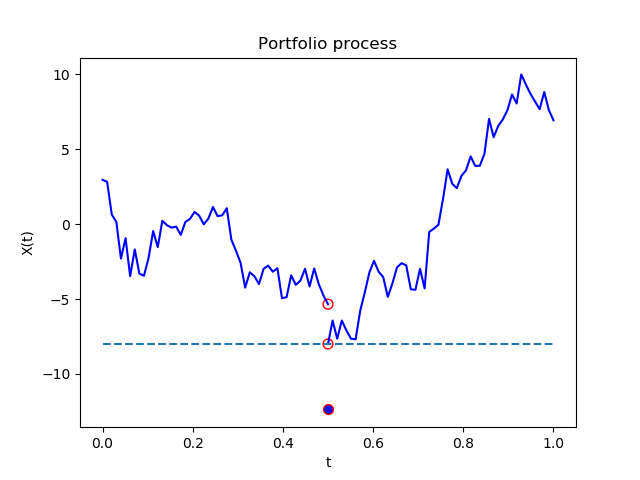
\includegraphics[scale=0.5]{./pics/portfolio_process.png}
 % wealth_process.png: 0x0 pixel, 300dpi, 0.00x0.00 cm, bb=
 \caption{Example of a discontinuous portfolio process $X^{\pi}(t)$ at time $t$. 
 The first jump is due to a jump in the process $S(t)$, the second jump is a consequence of the action on $B(t)$ and $Y(t)$ 
 of the left-continuous control $\pi(t)$. The dashed line divide the NT region from the buy/sell region.}
 \label{fig:portfolio process}
\end{figure}
Under this assumptions the processes $B^{\pi}(t)$ and $Y^{\pi}(t)$ are left-continuous, while the stock price process $S(t)$ is right-continuous. The portfolio process 
$X^{\pi}(t) = (B^{\pi}(t),Y^{\pi}(t),S(t))$ as well as the wealth process defined in 
(\ref{wealth_process}), are a combination of left-continuous and right-continuous processes, and therefore they can have purely discontinuous points.
In Figure \ref{fig:portfolio process} we present a simplified example of a portfolio, discontinuous in $t$, 
where the left limit and the right limit are both different from the value assumed by $X^{\pi}(t)$ in $t$.
\begin{Definition}
We define the \textbf{first exit time} from the solvency region $\SI^j$ as
\begin{equation}\label{exit_time}
 \tau^j = \inf \bigl\{ t \in [t_0,T] : \mathcal{W}^j_t \not\in \SI^j \bigr\}.
\end{equation} 
\end{Definition}
As long as we describe the underlying stock as a process with jumps, we cannot guarantee that the portfolio stays
solvent for all $t \in [t_0,T]$. Holding short positions, it is possible that a sudden increase in the value of the stock 
can cause the total wealth to jump instantaneously out of the solvency region. 
The same can happen with a downward jump when the investor is long in stocks and negative in cash. 
The sudden decrease of the stock's price makes him unable to pay his debts.
If the investor goes bankrupt, there are no trading strategies to save him.
\begin{Definition}\label{set_trading_strategies}
We define the set of \textbf{admissible trading strategies} $\Pi(B_0,Y_0,S_0)$,   
as the set of all left-continuous, nondecreasing, $\mathcal{F}_t$-adapted, progressively measurable processes  
$\pi(t): \Omega \times [t_0,T]\to \R^2$, such that the process $(B^\pi(t),Y^\pi(t),S(t))$ is a solution of (\ref{porfolio_dynamics}) 
with initial state $( B_0,Y_0,S_0 )$, and such that $\mathcal{W}^{\pi}(t) \in \SI^j$, for all $t\in [t_0,\tau^j)$. 
\end{Definition}
Basically, at time $t_0$, it is not possible to guarantee that the process never jumps out of the solvency region, and therefore we cannot impose the condition  
$\mathcal{W}^j_t \in \SI^j$ valid for all $t \in [t_0,T] $. \\
Remember that we are working with Markov controls, and therefore that at each time $t\in [t_0,T)$
we can express the control as a function of the current time and state: $\pi(t) = f(t,B_t,Y_t,S_t)$. 

To check that our definition is consistent, define $\bar t = s \wedge \tau$ for $s\in[t_0,T)$. As previously explained, the wealth process can be a discontinuous process, 
and if there is a
jump at time $\bar t$, in general we can have $\mathcal{W}^{\pi(\bar t^-)}(\bar t^-) \not = \mathcal{W}^{\pi(\bar t)}(\bar t) \not = \mathcal{W}^{\pi(\bar t^+)}(\bar t^+) $ with
$\pi(\bar t^-) = \pi(\bar t)$ (see for instance figure \ref{fig:portfolio process}). 
The control, in order to be admissible, have to keep the process inside the solvency region, $\mathcal{W}^{\pi(\bar t^+)}(\bar t^+) \in \SI$.
If $\bar t \geq \tau$, then $\mathcal{W}^{\pi}(\bar t) = \mathcal{W}^{\pi}(\tau)$ (the process is stopped) and therefore, $\mathcal{W}^{\pi(\bar t^+)}(\bar t^+) \not \in \SI$ whatever
control we choose.
The set of admissible trading strategies computed for a process starting in $(B_{\bar t},Y_{\bar t},S_{\bar t})$, with $\bar t \geq \tau$, 
is $\Pi(B_{\bar t},Y_{\bar t},S_{\bar t}) = \{ \emptyset \}$.
Once the process jumps out of the solvency region, there are no controls that can bring it back.\\
We will touch again this topic in Chapter \ref{Chapter6} when talking about the variable reduction.
\begin{Remark}
The original model formulated by \cite{HoNe89}, 
considers a portfolio starting with zero total wealth. 
It does not consider the possibility of insolvency.
The writer (or buyer) of the option creates a portfolio at time $t_0$ in order to hedge the option.
Therefore it is reasonable to assume that it does not own any shares in the underlying stock at time $t_0$. 
Following the literature, we consider a portfolio with zero initial shares and an initial amount $B_0$ in the 
cash account. This assumption can be easily relaxed to include an initial number $Y_0$ of shares if needed.
\end{Remark}

The investor wishes to maximize the expected utility of the wealth of his portfolio. 
\begin{align}\label{max_probl1}
V^j(t_0,B_0^j,Y_0,S_0) = \sup_{\pi \in \Pi(B_0^j,Y_0,S_0)} \;& \E_{B_0^j,Y_0,S_0}\biggl[ 
            \mathcal{U}(\mathcal{W}^j_T) \; \mathbbm{1}_{\{\tau^j > T\}} \\ \nonumber
             &+ e^{r(T-\tau^j)}\mathcal{U}(-C) \; 
             \mathbbm{1}_{\{\tau^j \leq T\}}\biggr], 
\end{align}
where $B_0^j$ is the initial cash amount in the no-option $j=0$, writer $(j=w)$ or buyer $(j=b)$ portfolio and can assume the values $B_0$, $B_0+p^w$ and $B_0-p^b$ respectively. 
The exit time $\tau^j$ is associated with the solvency region $ \mathcal{S}^j$, respectively for $j=0,w,b$.
The indicator functions separate the two cases of solvency at maturity date $T$, 
and bankruptcy at $\tau \leq T$. This feature is not present in the work of \cite{DaPaZa93}.
In the case of default the value function assumes the lowest possible
value attainable by $\mathcal{U}$, multiplied by the factor $e^{r(T-\tau^0)}$. 



The HJB equation associated to this stochastic control problem can be obtained with the same procedure used to derive (\ref{DPZ_HJB}). In this case the infinitesimal generator has the 
general form (\ref{inf_gen_exp_levy}) for exponential Lévy processes, and the variational inequality is
\begin{align}\label{HJB1}
& \max \; \biggl\{ \; \frac{\partial V^j}{\partial t} + rb\frac{\partial V^j}{\partial b} 
+ \mu s \frac{\partial V^j}{\partial s} + \frac{1}{2}\sigma^2 s^2 \frac{\partial^2 V^j}{\partial s^2} \\ \nonumber
&+ \int_\mathbb{R}
\biggl[ V^j(t,b,y,se^z) - V^j(t,b,y,s) - s(e^z-1)\frac{\partial V^j}{\partial s} \biggr] \nu(dz) \;,\\ \nonumber
& \;  \frac{\partial V^j}{\partial y}-(1+\theta_b) s \frac{\partial V^j}{\partial b} \; 
, \; -\biggl(\frac{\partial V^j}{\partial y}-(1-\theta_s)s \frac{\partial V^j}{\partial b} \biggr) \biggr\} = 0, 
 \end{align}
for $(t,b,y,s) \in [t_0,T) \times \SI^j$ and $j=0,w,b$.   
The main difference between this model and the previous models in the literature is that this HJB equation is a
partial integro-differential equation (PIDE), which involves an additional integral operator.
The presence of this non-local operator implies that 
we need to define the lateral conditions not only on the boundary
of the solvency region, but also beyond.
This is given by the condition
\begin{equation}\label{lat_conditions}
V^j(t,b,y,s) = e^{r(T-t)} \mathcal{U}(-C) \hspace{1em} \mbox{ for } \hspace{1em} 
t \in [t_0,T] , \hspace{0.5em} (b,y,s) \not \in \mathcal{S}^j, \hspace{1em} j=0,w,b.
\end{equation}
The terminal condition is
\begin{equation}\label{terminal_conditions}
V^j(T,b,y,s) = \mathcal{U}\bigl( w^j(b,y,s) \bigr) \hspace{1em} \mbox{ for } \hspace{1em} 
t \in [t_0,T] , \hspace{0.5em} (b,y,s) \in \mathcal{S}^j 
\end{equation}
with
\begin{itemize}
  \item No option: 
  \begin{equation*}
   w^0(b,y,s) =  b + c(y,s).
  \end{equation*}
  \item Writer: 
  \begin{equation*}
   w^w(b,y,s) =  b + c(y,s) \mathbbm{1}_{\{ c(1,s) \leq K\}} +
  \biggl( c\bigl( y-1,s \bigr) + K \biggr) \mathbbm{1}_{\{c(1,s)>K\}}.
  \end{equation*}
  \item Buyer: 
  \begin{equation*}
   w^b(b,y,s) = b + c(y,s) \mathbbm{1}_{\{ c(1,s) \leq K\}} +
  \biggl( c\bigl( y+1,s \bigr) - K \biggr) \mathbbm{1}_{\{c(1,s)>K\}}.
  \end{equation*}
\end{itemize}









\section{Existence of viscosity solution}

The general fact that value functions of control problems can be characterized as
viscosity solutions of certain partial differential equations is a direct consequence of the dynamic
programming principle. For singular control problems, however, the classical approach of Lions
fails because the state process may jump due to the singular control and it needs thus not stay
in a small ball for small t. This problem has been circumvented in the previous works in the literature, by relying on the
existence of the optimal control (see e.g. \cite{DaPaZa93}).
In our approach, we bypass this technical problem by approximating the singular left-continuous control with a sequence of continuous controls (see Remark (\ref{RemarkDPZ})).\\ 
Another difficulty that arise in our proof is the presence of jumps in the uncontrolled dynamics.
The existence proof (usually in the subsolution part) frequently makes use of stopping times to ensure that a stochastic
process $X_t$, started at $x$, is contained in some small set. This works very well for
continuous processes, because then for a stopping time 
\begin{equation}
 \tau = \inf\{ s \geq 0 : |X_s - x| \geq \rho \} \wedge t 
\end{equation}
with $\rho >0$, the condition $|X_{\tau} - x| \leq \rho$ always holds. For a process including (non-predictable) jumps however,
$|X_{\tau} - x|$ may be greater than $\rho$. Luckily, Lévy processes and, more in general, all the controlled processes with dynamics as in Eq. (\ref{controlled_SDE}), 
are \textbf{stochastically continuous}, which
means that the probability of $X_{\tau}$ being outside $\mathcal{B}(x, \rho )$ converges to zero, if $t\to 0$.
\begin{Theorem}\label{stochastic_theorem}
 A process $X_t$ starting at $X_0=x$ and with dynamics as in Equation (\ref{controlled_SDE}), for each $ \alpha \in \mathcal{A}$\footnote{The control set is defined
 as in Section \ref{Optimal_control_framework}. This theorem does not hold when $\alpha: [0,T]\times \Omega \to A$ with $A$ unbounded.}, and for each $\rho>0$, satisfies
 \begin{equation}
   \PP \biggl( | X_t - x | \geq \rho \biggr) \to 0 \quad \mbox{ as } \quad t\to0.
 \end{equation}
\end{Theorem}
\begin{proof}
By the Markov inequality
 \begin{align*}
  \PP \biggl( | X_t - x | \geq \rho \biggr) & \leq \frac{\E_{\bar x}\biggl[ |X_t - \bar x| \biggr]}{\rho} \\
   & \leq \frac{C}{\rho} (1+|x|)\sqrt{t}
 \end{align*}
 where we used (\ref{cond_2}), with $C>0$. Taking the limit $t\to 0$ proves the theorem.
\end{proof}
   
Let us restrict our attention on the subset $\mathcal{A}^k$ of all the absolute continuous controls $L(t), M(t) \in \Pi(X_0)$, as done previously in Section
\ref{subsec_HJB}. 
Using (\ref{absolute_cont_controls}), the portfolio process $X^{\pi}_t=(B^{\pi}_t, Y^{\pi}_t, S_t)$ with equation (\ref{porfolio_dynamics}) is approximated by $X^k_t$ with dynamics:
\begin{equation}\label{porfolio_dynamics3}
 \begin{cases}
 dB^{k}_t &=  rB_t dt - (1+\theta_b)S_t l_t\, dt + (1-\theta_s) S_t m_t\, dt \\
 dY^{k}_t &=  (l_t - m_t)dt \\
 dS_t &=  S_t \left( \mu dt + \sigma dW_t + \int_{\R} (e^z-1) \tilde N(dt,dz) \right).
\end{cases}
\end{equation} 
where $0 \leq l_t \leq k$ and $0 \leq m_t \leq k$ with $k<\infty$.\\
In order to clarify, let us consider an example of a left-continuous control that is the point-wise limit of a sequence of continuous controls.\\ 
\textbf{Example:}\\
Assume that at time $t_0=0$ the portfolio is in the buy region. Therefore the control moves the portfolio inside the NT region, for instance by buying one share $\Delta L(0) = 1$. 
Assume also, for simplicity, that the portfolio never exits
the NT region in $(0,T]$, such that the control is constant in $(0,T]$. The control $L(t)$ has the form:
\begin{equation}
L(t) = 
 \begin{cases}
  0 \quad \mbox{ for } \quad t = 0\\  
  1 \quad \mbox{ for } \quad t \in (0,T]
 \end{cases}
\end{equation}
Define the sequence:
\begin{equation}
L^k(t) = 
 \begin{cases}
  k t \quad \mbox{ for } \quad t \in [0,\frac{1}{k}] \\  
  1 \quad \mbox{ for } \quad t \in (\frac{1}{k},T]
 \end{cases}
\end{equation}
where $l_t = k$.
For $k\to \infty$ the sequence of continuous functions $L^k(t)$ converges point-wise to the left-continuous function $L(t)$.\\

Let us call $\tau_{\SI}$ the first exit time from $\SI$.
Since the exponential Lévy process that governs the dynamics of $S_t$ is stochastically continuous,
it is possible to exclude an immediate jump in $X_t$, i.e. $t_0 = \tau_{\SI}$, which may cause bankruptcy.
Moreover, we can apply the theorem (\ref{stochastic_theorem}) to guarantee that for every fixed $k>0$, the process $X^k_t$ can be contained in a small ball.  
More precisely, for every $x \in \SI$, 
we can always find a $\rho>0$ such that the ball $\mathcal{B}(x, \rho) \in \SI$, and call $\tau^{\rho} < \tau_{\SI}$ the first exit time from it.   
Then for $t_0 < t < \tau^{\rho}$, we obtain that $$\PP( X^k_{t} \in \mathcal{B}(x, \rho) | X^k_{t_0} = x) \to 1 \quad \mbox{ as } t \to t_0.$$

In this section we prove that the value function of the singular stochastic control problem with jumps, presented in the previous section, can be interpreted 
as the viscosity solution of the HJB equation associated to the problem.
In our proof, unlike the proof of \cite{DaPaZa93}, we do not assume the existence of an optimal control. 
However, as in \cite{DaPaZa93} we assume the continuity of the value function, and refer to the continuity proof presented in \cite{Ph98}. 
Some references that prove the continuity of the value function, considering continuous processes, are 
\cite{ShSo94}, \cite{Pham}, \cite{Damgaard}. All these proofs rely on the fact that the utility function is concave. After proving that value function is concave 
as well, the continuity follows as a consequence.  
In \cite{OkSu01}, the authors use the same approach to prove the continuity of the value function when the portfolio dynamics has jumps. 
However they don't consider the possible exit from the solvency region. 
We consider the following more general theorem, presented and proved in \cite{Ph98} (Proposition 3.3).
\begin{Theorem}\label{continuity_VF}
 Under assumptions  (\ref{Lipschitz_control}),(\ref{Lipschitz_control2}), (\ref{Growth_control}), (\ref{Growth_control2}), (\ref{Lipschitz_f}) and \ref{linear_growth_f}, 
 the value function \ref{general_value_function} is continuous. 
\end{Theorem}
The author uses the Lipschitz condition (\ref{Lipschitz_f}) to prove that the value function is continuous in $x$, and the dynamic programming principle to prove that it is continuous
in $t$. The theorem in \cite{Ph98} is even more general, because it permits to consider a maximization over all stopping time as well.\\
This theorem can be applied to the maximization problem \ref{max_probl1}, since all its hypothesis are verified.
\newline
\noindent
First of all we have to interpret the HJB equation (\ref{HJB1}), (\ref{lat_conditions}), (\ref{terminal_conditions}) in terms of the general theory for parabolic problems 
(\ref{parabolic_PIDE}). 
We use the dummy variable $x = (b,y,s)$ to indicate a point in $\R^2\times \R^+$. In order to satisfy the elliptic and parabolic conditions we rewrite the  HJB as 
\begin{align}\label{HJB2}
& \min \; \biggl\{ - \biggl( \; \frac{\partial V}{\partial t} + rb\frac{\partial V}{\partial b} 
+ \mu s \frac{\partial V}{\partial s} + \frac{1}{2}\sigma^2 s^2 \frac{\partial^2 V}{\partial s^2} \\ \nonumber
&+ \int_\mathbb{R}
\biggl[ V(t,b,y,se^z) - V(t,b,y,s) - s(e^z-1)\frac{\partial V}{\partial s} \biggr] \nu(dz) \; \biggr) ,\\ \nonumber
& \; - \biggl( \frac{\partial V}{\partial y}-(1+\theta_b) s \frac{\partial V}{\partial b} \biggr) \; 
, \; + \biggl(\frac{\partial V}{\partial y}-(1-\theta_s)s \frac{\partial V}{\partial b} \biggr) \biggr\} = 0, 
\end{align}
and this corresponds to   
$ F(t,x,V,D_t V,D_x V,D_{xx}V,\I(t,x,V)) = 0$ in the domain $(t,x) \in [t_0,T) \times \SI$.
To simplify the notation, let us introduce the integro-differential infinitesimal generator:
\begin{align*}
 \LL V(t,x) &= -\biggl( \frac{\partial V}{\partial t}(t,x) + rb\frac{\partial V}{\partial b}(t,x) 
  + \mu s \frac{\partial V}{\partial s}(t,x) + \frac{1}{2}\sigma^2 s^2 \frac{\partial^2V}{\partial s^2}(t,x)\biggr) \\
  &- \int_{\R}
[ V(t,b,y,se^z) - V(t,b,y,s) - s(e^z-1)\frac{\partial V}{\partial s} ] \nu(dz),
\end{align*}
such that $F\Bigl(t,x,V,D_t V,D_x V,D_{xx}V,\I(t,x,V)\Bigr) = 0$ has the form
\begin{equation}\label{qvi_min}
  \min \; \biggl\{ \; \LL V(t,x),
  \, -(V_y-(1+\theta_b)sV_b) \, , \; V_y-(1-\theta_s)s V_b \biggr\} = 0.
\end{equation}
In order to prove that $V(t,x)$ is a viscosity solution we need to verify both the subsolution and supersolution properties.



\subsection{Subsolution}

In this section we prove that the value function can be interpreted as a viscosity subsolution of the HJB equation associated to the maximization problem. 
We enunciate the following theorem:
\begin{Theorem}\label{subsolution_th}
 The value function of the maximization problem (\ref{max_probl1}), is a viscosity subsolution of the Eq. (\ref{qvi_min}).
\end{Theorem}
\begin{proof}
Thanks to the continuity property of the value function (see theorem (\ref{continuity_VF})), for any $(t, x) \not \in [t_0,T) \times \SI$ we immediately see that 
the subsolution property (\ref{subsolution}) is verified.
We now want to prove that $V(t, x)$ is a subsolution for $(t, x) \in [t_0,T) \times \SI$.

Let us consider a test function $ \phi \in C^2([t_0,T] \times \R^2\times \R^+) \bigcap \mathcal{C}_2([t_0,T] \times \R^2\times \R^+)$ such that 
$(\bar t,\bar x)$ is a maximum point for $V-\phi$:
\begin{equation}
 V(\bar t,\bar x) - \phi(\bar t,\bar x) \geq V(t,x) - \phi(t, x) \hspace{2em} \forall (t,x) \in [t_0,T) \times \SI
\end{equation}
and we assume without loss of generality that:
\begin{equation}\label{max_point}
V(\bar t,\bar x) = \phi(\bar t,\bar x)  
\end{equation}
so we can write:
\begin{equation}\label{max_point2}
V(t,x) \leq \phi(t, x) 
\end{equation}
We want to prove that
$$ F(\bar t,\bar x,V(\bar t, \bar x),D_t \phi(\bar t, \bar x),D_x \phi(\bar t, \bar x),D_{xx}\phi(\bar t, \bar x),
\I(\bar t, \bar x,\phi(\bar t, \bar x))) \leq 0  $$
\textbf{Reductio ad absurdum:}\\
Let us assume that 
$$F(\bar t,\bar x,V(\bar t, \bar x),D_t \phi(\bar t, \bar x),D_x \phi(\bar t, \bar x),D_{xx}\phi(\bar t, \bar x),
\I(\bar t,\bar x,\phi(\bar t, \bar x))) >0.$$ 
This means that all the terms inside the minimum in Eq. (\ref{qvi_min}) are positive, i.e. exist $\kappa_1, \kappa_2, \kappa_3 >0$ such that:
\begin{enumerate}
 \item $ \LL \phi(\bar t, \bar x) > \kappa_1 ,$
 \item $-\left(\frac{\partial \phi}{\partial y}(\bar t, \bar x)
 -(1+\theta_b)s \frac{\partial \phi}{\partial b}(\bar t, \bar x)\right) > \kappa_2,$
 \item $\frac{\partial \phi}{\partial y}(\bar t, \bar x)-(1-\theta_s)s \frac{\partial \phi}{\partial b}(\bar t, \bar x) > \kappa_3.$
\end{enumerate}
Since the test function is smooth by definition, there exist a ball $\mathcal{B}(\bar x, \rho) \in \SI$ 
where the previous conditions are satisfied $\forall x \in \mathcal{B}(\bar x, \rho)$. 
We define also the exit time from the ball $\mathcal{B}(\bar x, \rho)$ for the approximated portfolio process $X^{k}_t$ introduced in (\ref{porfolio_dynamics3})
\begin{equation}
 \tau_{\rho} = \inf \{ t \in [t_0,T] : X^{k}_t \not \in \mathcal{B}(\bar x, \rho) \}
\end{equation}
such that $\tau_{\rho} < \tau_{\SI}$.\\

By the DPP (\ref{DPP2}), for all $\tau \in \mathcal{T}_{\bar t,\tau_{\rho}}$ and for all $\epsilon > 0$, there exists $\pi(\cdot) \in \mathcal{A}^k(\bar t,\bar x)$ such that
\begin{equation}
  V(\bar t, \bar x) \leq \E_{\bar x} \Bigl[ V(\tau, X^{k}(\tau)) \Bigr] +\epsilon.
\end{equation}
Using (\ref{max_point}) and (\ref{max_point2}) we can write:
\begin{equation*}
 \phi(\bar t, \bar x) = V(\bar t, \bar x) \; \leq \E_{\bar x}[V(\tau, X^{k}(\tau))] + \epsilon \; 
 \leq \E_{\bar x}[\phi(\tau, X^{k}(\tau))] + \epsilon.
\end{equation*}
Let us call $\tau = \bar t + h$, and choose a $\tau$ small enough such that we can write 
$$\phi \bigl( \bar t +h, X^{k}(\bar t+h)\bigr) = \phi(\bar t, \bar x) + d\phi(\bar t, \bar x), $$ 
with
$L(\bar t+h) = L(\bar t) + l(\bar t)\,h$ and $M(\bar t +h) = M(\bar t) + m(\bar t)\,h$ and $0 \leq l(\bar t),m(\bar t) \leq k$ for any fixed $k>0$.\footnote{For each fixed $k$, 
it is always possible to choose a $\tau$ small enough such that the process does not exit the ball $\mathcal{B}(\bar x, \rho)$ a.s.}
\begin{align}\label{first_inequality2}
 0 \; \leq & \; \E_{\bar x} \biggl[ \phi(\bar t +h, X^{k}(\bar t+h)) - \phi(\bar t, \bar x) \biggr] +\epsilon \\ \nonumber
   \leq & \; \E_{\bar x} \biggl[ \biggl( -\LL \phi(\bar t, \bar x) + \left(\frac{\partial \phi}{\partial y}(\bar t, \bar x)
 -(1+\theta_b)s \frac{\partial \phi}{\partial b}(\bar t, \bar x)\right) l(\bar t) \\ \nonumber
   & - \left( \frac{\partial \phi}{\partial y}(\bar t, \bar x)-(1-\theta_s)s \frac{\partial \phi}{\partial b}(\bar t, \bar x) \right) m(\bar t) \biggr)\; h \biggr] + \epsilon.\\ \nonumber
   <& \underbrace{\biggl( -\kappa_1 - \kappa_2\, l(\bar t) - \kappa_3\, m(\bar t) \biggr) \, \E_{\bar x} \bigl[ h \bigr]}_{<0} + \epsilon. 
\end{align}
Since this must hold true for all $\epsilon$, when taking the limit $\epsilon \to 0$ we get a contradiction.
\end{proof}





\subsection{Supersolution}

Following the previous section, we now want to prove that the value function is a viscosity supersolution of the HJB equation (\ref{qvi_min}). 

\begin{Theorem}\label{supersolution_th}
 The value function of the maximization problem (\ref{max_probl1}), is a viscosity supersolution of the Eq. (\ref{qvi_min}).
\end{Theorem}

\begin{proof}
Since the value function $V \in C^0([t_0,T]\times \R^2\times \R^+)$, it is straightforward to verify that for any $(t, x) \not \in [t_0,T) \times \SI$
the supersolution property (\ref{supersolution}) immediately hold.
Let us prove that $V(t, x)$ is a supersolution for $(t, x) \in [t_0,T) \times \SI$.

Let us consider a test function $ \phi \in C^2([t_0,T] \times \R^2\times \R^+) \bigcap \mathcal{C}_2([t_0,T] \times \R^2\times \R^+)$ such that 
$(\bar t,\bar x)$ is a minimum point for $V-\phi$.\\
\begin{equation}
 V(\bar t,\bar x) - \phi(\bar t,\bar x) \leq V(t,x) - \phi(t, x) \hspace{2em} \forall (t,x) \in [t_0,T) \times \SI
\end{equation}
and we assume without loss of generality that:
\begin{equation}\label{min_point}
V(\bar t,\bar x) = \phi(\bar t,\bar x)  
\end{equation}
so we can write:
\begin{equation}\label{min_point2}
V(t,x) \geq \phi(t, x) 
\end{equation}
We want to prove that
$$ F(\bar t,\bar x,V(\bar t, \bar x),D_t \phi(\bar t, \bar x),D_x \phi(\bar t, \bar x),D_{xx}\phi(\bar t, \bar x),
\I(\bar x,\phi(\bar t, \bar x))) \geq 0  $$
that is analogous to prove that all the following terms are non-negative.
\begin{enumerate}
 \item 
 $ \LL \phi(\bar t, \bar x) \geq 0 ,$
 \item $-\left(\frac{\partial \phi}{\partial y}(\bar t, \bar x)
 -(1+\theta_b)s \frac{\partial \phi}{\partial b}(\bar t, \bar x)\right) \geq 0,$
 \item $\frac{\partial \phi}{\partial y}(\bar t, \bar x)-(1-\theta_s)s \frac{\partial \phi}{\partial b}(\bar t, \bar x) \geq 0.$
\end{enumerate}

By the DPP (\ref{DPP1}), for all $\tau \in \mathcal{T}_{\bar t,\tau_{\rho}}$ and for all $\pi(\cdot) \in \Pi(X_{\bar t})$, we can write:\footnote{Since this holds for 
all $\pi(\cdot) \in \Pi(X_{\bar t})$ we can restrict our attention to the controls such that $0 \leq \Delta L(\bar t) < \rho $ and $0 \leq \Delta M(\bar t)) < \rho$.}
\begin{equation}
  V(\bar t, \bar x) \geq \E_{\bar x} \Bigl[ V(\tau, X^{\pi}(\tau)) \Bigr].
\end{equation}
Using (\ref{min_point}) and (\ref{min_point2}) we can write:
\begin{equation*}
 \phi(\bar t, \bar x) = V(\bar t, \bar x) \; \geq \E_{\bar x}[V(\tau, X^{\pi}(\tau))] \; 
 \geq \E_{\bar x}[\phi(\tau, X^{\pi}(\tau))]
\end{equation*}
Let us call $\tau = \bar t + h$. The test function $\phi$ is smooth enough to use the generalized Dynkin formula.
\begin{align}\label{first_inequality}
 0 \; \geq & \; \E_{\bar x} \biggl[ \phi(\bar t +h, X^{\pi}(\bar t+h)) \biggr] - \phi(\bar t, \bar x) \\ \nonumber
   \geq & \; \E_{\bar x} \biggl[ \int_{\bar t}^{\bar t +h} \biggl[ -\LL \phi(t,X_t) + \biggl( \phi \bigl( t^+, B_t - (1+\theta_b) S_t\, dL_t, Y_t + dL_t, S_t \bigr) 
     - \phi \bigl(t,X_t \bigr) \biggr) \\
   & + \biggl( \phi \bigl( t^+, B_t + (1-\theta_s) S_t\, dM_t, Y_t - dM_t, S_t \bigr) - \phi \bigl( t,X_t \bigr) \biggr) \biggr] dt \biggr]
\end{align}
where with $t^+$ we indicate that $\phi \bigl( t^+, B_t - (1+\theta_b) S_t\, dL_t, Y_t + dL_t, S_t \bigr)$ is 
the right limit $\lim_{u \downarrow t} \phi \bigl( u, B_u, Y_u, S_u \bigr)$ (remember that $B_t$ and $Y_t$ are left continuous).\\
Now we can consider the two cases:
\begin{enumerate}
 \item $\Delta \pi(\bar t)>0$. Let us assume for instance that $\Delta L(\bar t)>0$ and $\Delta M(\bar t)=0$. 
 \item $\Delta \pi(\bar t)=0$. This means that the control is continuous in $\bar t$: since $\Delta \pi(\bar t) = 0$, we obtain $L(\bar t^+) = L(\bar t)$ and
 $M(\bar t^+) = M(\bar t)$.   
\end{enumerate}
Let us consider the first case.
Taking the limit $h \to 0$ and writing $\bar x = (\bar b, \bar y, \bar s)$ we obtain the following expression
\begin{equation*}
 0 \geq \phi \bigl( \bar t^+, \bar b - (1+\theta_b) \bar s\, \Delta L(\bar t), \bar y + \Delta L(\bar t), \bar s \bigr) - \phi(\bar t, \bar b, \bar y, \bar s),
\end{equation*} 
The term $\lim_{h\to 0} \int_{\bar t}^{\bar t +h} - \LL \phi(t,X(t)) dt \to 0$, since the uncontrolled process $X(t)$ is right-continuous and $\LL \phi(\cdot)$ is continuous, 
the term $\LL \phi(t,X(t))$ is right-continuous as well.\\  
The previous equation is true for all $\Delta L(\bar t)>0$, so we can take the limit $\Delta L(\bar t) \to 0$ and get
\begin{equation*}
 \frac{\partial \phi}{\partial y}(\bar t, \bar x)
 -(1+\theta_b) \bar s \frac{\partial \phi}{\partial b}(\bar t, \bar x) \leq 0,
\end{equation*}
and then multiplying by -1, we obtain the point (2). 
\begin{equation*}
-\left(\frac{\partial \phi}{\partial y}(\bar t, \bar x)
 -(1+\theta_b) \bar s \frac{\partial \phi}{\partial b}(\bar t, \bar x)\right) \geq 0.
\end{equation*}
Choosing instead $\Delta M(\bar t)>0$ and $\Delta L(\bar t)=0$ and following the same reasoning, we obtain the point (3).\\

\noindent
Now consider the second case where $\Delta \pi(\bar t)= (\Delta L(\bar t),\Delta M(\bar t)) =0$.
We can choose a stopping time $\tau$ such that all the controls in $[\bar t, \tau]$ are continuous. We also assume, for simplicity, constant controls, i.e.
$dL_t = dM_t = 0$ for all $t \in [\bar t, \tau]$.\\
The equation (\ref{first_inequality}) becomes 
\begin{equation*}
 \int_{\bar t}^{\bar t +h} - \LL \phi(t,X_t) dt \leq 0.
\end{equation*}
Let us divide by $h$, sent $h\to 0$ and use the mean value theorem to get:
\begin{equation*}
 \LL \phi(\bar t, \bar x) \geq 0,
\end{equation*}
proving the point (1).
\end{proof}


\noindent
We conclude this Chapter with the following main theorem:
\begin{Theorem}
 The value function of the maximization problem (\ref{max_probl1}), is a viscosity solution of the Eq. (\ref{qvi_min}).
\end{Theorem}
The proof is a direct consequence of theorems \ref{subsolution_th} and \ref{supersolution_th}. Since the value function is both a viscosity 
subsolution and a supersolution, it is a viscosity solution.


